\chapter{Design}
\label{chap:design}

To ensure a robust and scalable architecture, we adopted the Model-View-Controller
(MVC) pattern along with a three-tier physical architecture. This approach
enhances modularity, maintainability, and scalability, making it easier to
develop and manage both the research pipeline and the operational deployment
of the forecasting system.

\section{MVC Model}
\label{sec:mvc}

The Model-View-Controller (MVC) pattern is a well-established architectural
design that promotes the separation of application concerns. It divides the
system into three distinct components:

\begin{itemize}
  \item \textbf{Model:} Responsible for managing the application's data,
        business logic, and machine learning computation. 

  \item \textbf{View:} Handles the presentation layer and defines how
        information is displayed to the user. 

  \item \textbf{Controller:} Acts as an intermediary between the model
        and the view, processing user requests and orchestrating the
        system workflow. 
\end{itemize}

The decision to adopt the MVC pattern stems from its key advantages:
separation of concerns improves code maintainability and facilitates
independent testing of each layer; reusability enables PyTorch modules
to be swapped between experiment configurations without modifying the
controller or view layers; modularity allows parallel development of the
frontend dashboard and the ML training pipeline; and testability is
simplified because each \texttt{nn.Module} can be unit-tested independently
with synthetic tensors before integration into the full pipeline.

In the context of our probabilistic demand forecasting system, the MVC
architecture is implemented as follows:

\begin{itemize}
  \item \textbf{Model layer:}
  \begin{itemize}
    \item Handles the processing of EMHIRES demand time series, exogenous
          feature encoding, quantile-level conditioning, and the storage
          of model checkpoints.
    \item All neural network components inherit from PyTorch's
          \texttt{nn.Module} and are serialised via \texttt{torch.save()}.
    \item The CQRCalibrator module wraps any trained backbone and applies
          conformal adjustment without modifying the underlying weights.
  \end{itemize}
  \item \textbf{View layer:}
  \begin{itemize}
    \item React with TypeScript provides a
          type-safe, component-based SPA with Tailwind CSS + PostCSS
          for styling, Radix UI and MUI for accessible UI widgets,
          Lucide React and MUI icons, Motion for animations, and
          next-themes for light/dark mode switching.
    
  \end{itemize}
  \item \textbf{Controller layer:}
  \begin{itemize}
    \item YAML configuration files and the PyTorch Lightning
        \texttt{Trainer} serve as the research controller. A Python FastAPI
        REST backend serves as the operational controller, routing forecast
        requests to the appropriate model checkpoint.
  \end{itemize}
\end{itemize}

\section{Physical Architecture}
\label{sec:physical}

The system follows a three-tier architecture, a widely adopted design pattern
for distributed applications. This architecture promotes separation of concerns
by organizing the system into three distinct layers:

\begin{itemize}
  \item \textbf{Presentation Tier:} The front-end interface through which
        users interact with the system, implemented using React 18+ with
        TypeScript and TailwindCSS. Communicates with the application
        backend through asynchronous REST API calls. The Plotly.js library
        provides the interactive time-series visualisation components.

  \item \textbf{Logic Tier:} The middle layer responsible for processing
        forecast requests, enforcing business rules, and coordinating
        model inference workflows. Implemented using Python FastAPI,
        exposing RESTful endpoints. 

  \item \textbf{Data Tier:} The back-end layer responsible for data
        persistence and retrieval. Utilises PostgreSQL 15+ as the primary
        relational database, Redis for in-memory caching and async job
        queuing, and the local filesystem for model checkpoint storage.
\end{itemize}

In our forecasting system, the three-tier architecture is realised as follows:

As shown in Figure~\ref{fig:package}, the Presentation Tier (React 18/Next.js,
TailwindCSS, Plotly.js) communicates with the Logic Tier (Uvicorn/FastAPI,
Celery/Redis async, JWT authentication), which coordinates with the
Machine Learning Engine (PyTorch Lightning/N-BEATS, GluonTS, OmegaConf)
and the Database Tier (PostgreSQL 15, Redis Cache, TimescaleDB). This
design ensures clear separation of responsibilities, scalability, and
long-term maintainability.

\section{Detailed Conception}
\label{sec:detailed}

The detailed conception phase focuses on providing a clear and structured
overview of the system's architecture and components through high-level
UML models.

\subsection{Object Sequence Diagram}
\label{subsec:object_seq}

In this section we focus on the most important sequence diagram at the
object level. Figure~\ref{fig:obj_seq} represents the sequence diagram
for the \textbf{forecast generation use case}, showing the detailed
object-level message exchanges during a complete inference cycle.

\begin{figure}[H]
  \centering
  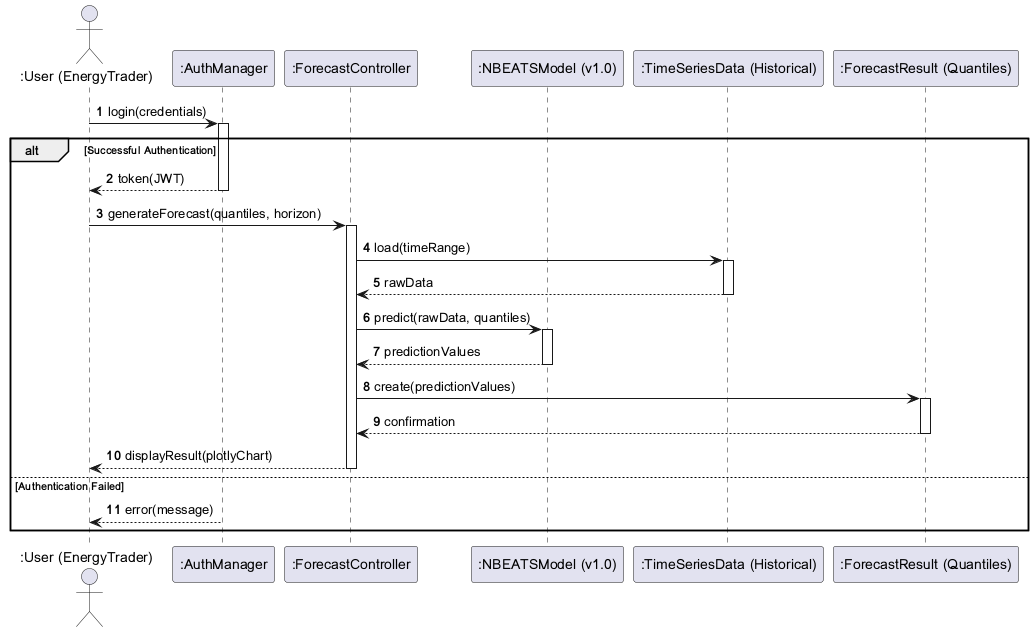
\includegraphics[width=\textwidth]{images/object_sequence_diagram_en (1).png}
  \caption{Object Sequence Diagram for the forecast generation use case.}
  \label{fig:obj_seq}
\end{figure}

\subsection{Activity Diagram}
\label{subsec:activity}

An activity diagram visually maps out a process from its initiation to
its completion, detailing the sequence of actions and explicitly presenting
all potential decision points, illustrating the various paths the process
can take as events unfold. Figure~\ref{fig:activity} shows our activity
diagram for the forecasting system workflow.

\begin{figure}[H]
  \centering
  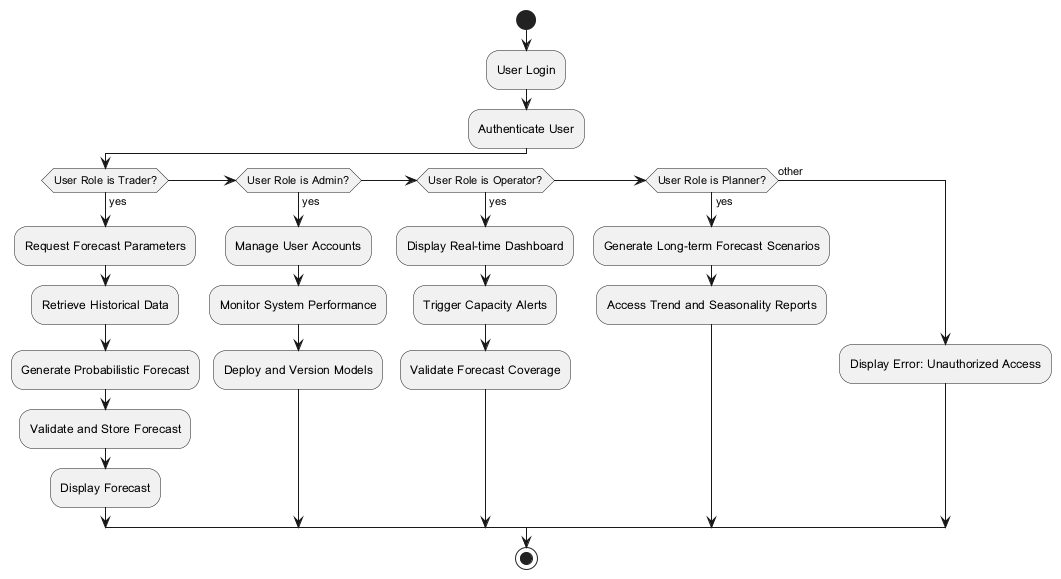
\includegraphics[width=\textwidth]{images/activity_diagram_en (1).png}
  \caption{Activity Diagram of the forecasting system workflow.}
  \label{fig:activity}
\end{figure}


\subsection{Package Diagram}
\label{subsec:package}

This UML package diagram illustrates a structured and modular system
architecture divided into four key layers. Figure~\ref{fig:package}
presents the complete package architecture of the Electricity Demand
Forecasting System.

\begin{figure}[H]
  \centering
  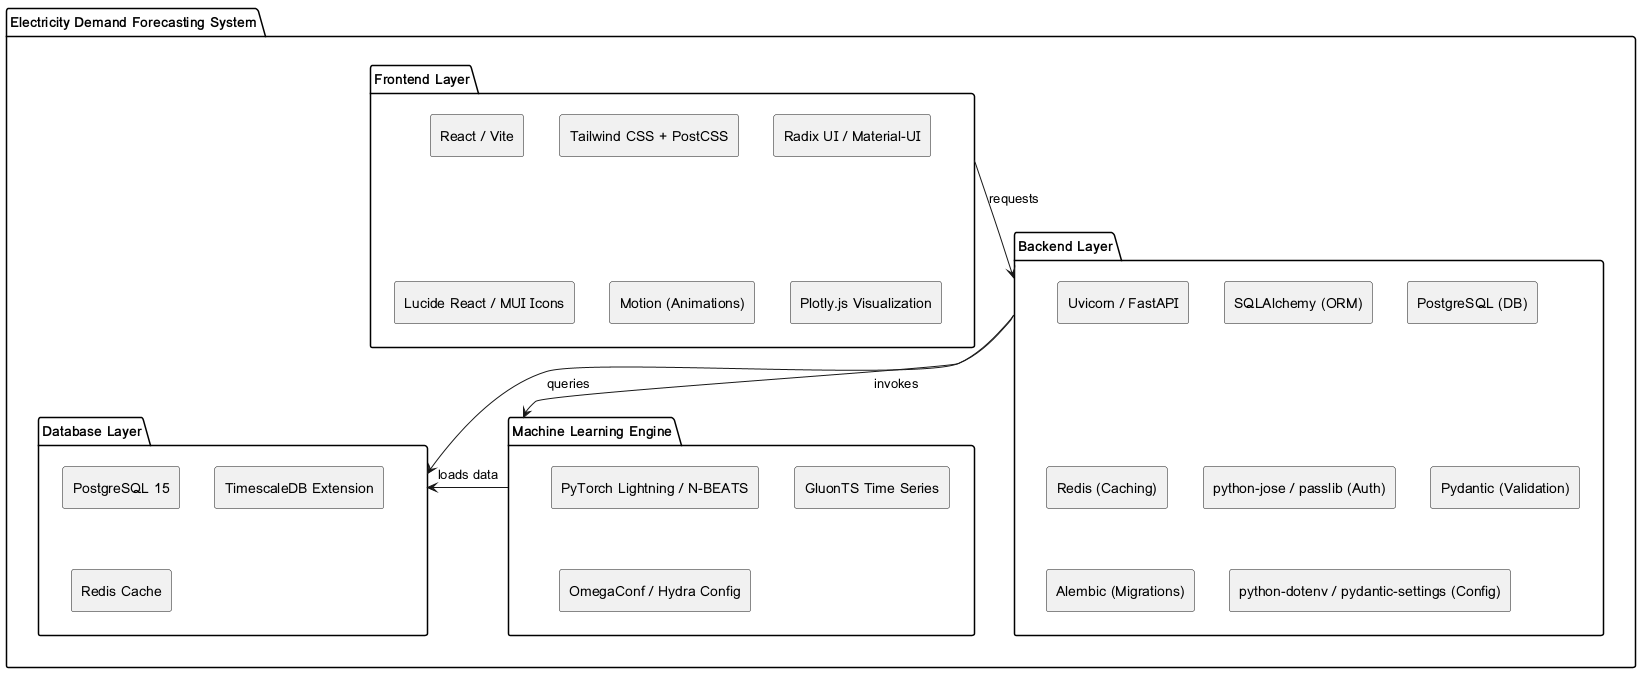
\includegraphics[width=\textwidth]{images/package_diagram_en (2).png}
  \caption{Package Diagram of the Electricity Demand Forecasting System.}
  \label{fig:package}
\end{figure}

\subsection{Class Diagram}
\label{subsec:class}

In our system design, we employed a UML class diagram to visualize the
architecture, relationships, and functionalities of key components.
Figure~\ref{fig:classdiag} illustrates the UML class diagram with its
main components and associations.

\begin{figure}[H]
  \centering
  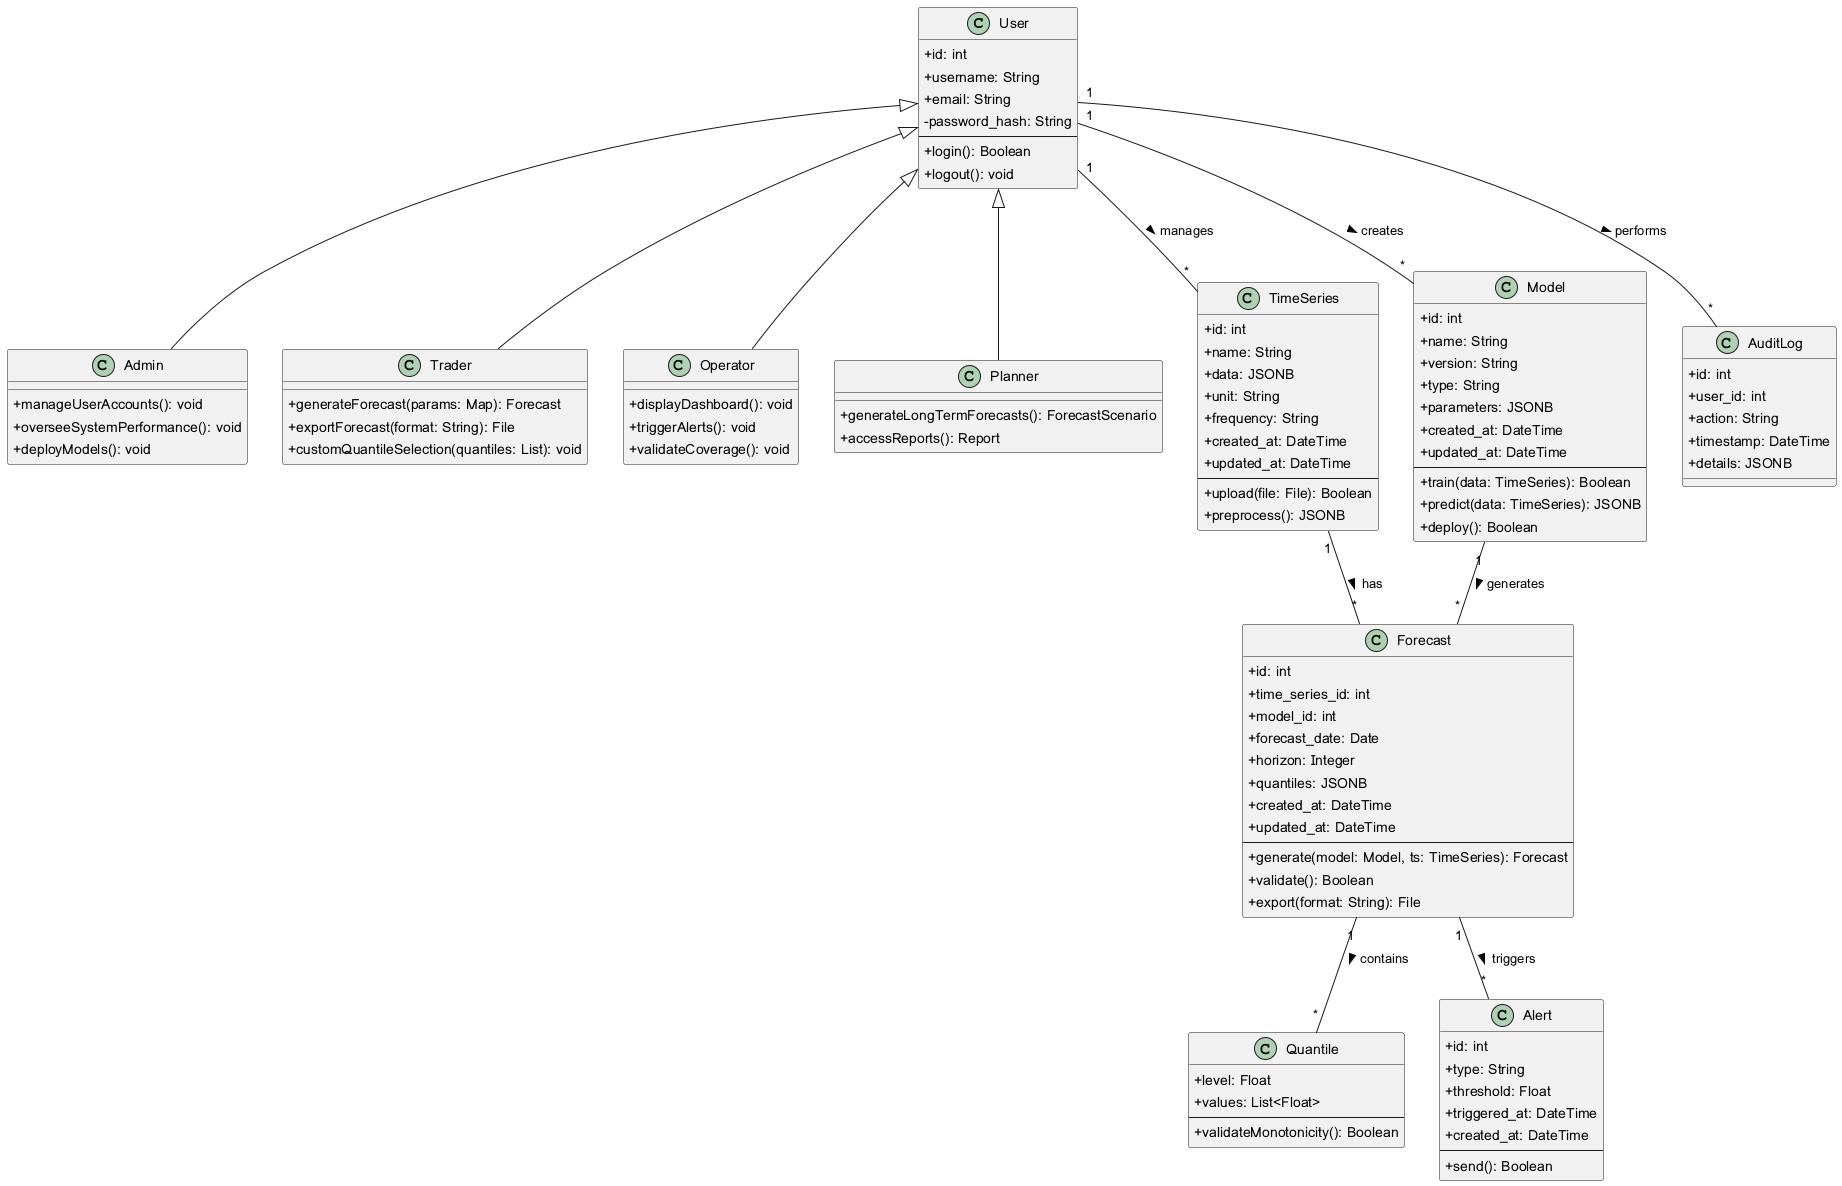
\includegraphics[width=\textwidth]{images/class_diagram_en (2).png}
  \caption{Class Diagram of the Electricity Demand Forecasting System.}
  \label{fig:classdiag}
\end{figure}

